\documentclass[12pt,letterpaper]{article}
\usepackage[utf8]{inputenc}
\usepackage[spanish, es-tabla]{babel}
\usepackage[version=3]{mhchem}
\usepackage[journal=jacs]{chemstyle}
\usepackage{amsmath}
\usepackage{amsfonts}
\usepackage{amssymb}
\usepackage{makeidx}
\usepackage{xcolor}
\usepackage[stable]{footmisc}
\usepackage[section]{placeins}
%Paquetes necesarios para tablas
\usepackage{longtable}
\usepackage{array}
\usepackage{xtab}
\usepackage{multirow}
\usepackage{colortab}
\usepackage{caption}
\usepackage{enumitem}
%Paquete para el manejo de las unidades
\usepackage{siunitx}
\sisetup{mode=text, output-decimal-marker = {,}, per-mode = symbol, qualifier-mode = phrase, qualifier-phrase = { de }, list-units = brackets, range-units = brackets, range-phrase = --}
\usepackage{cancel}
%Paquetes necesarios para imágenes, pies de página, etc.

%Instrucción para evitar la indentación
%\setlength\parindent{0pt}
%Paquete para incluir la bibliografía
\usepackage[backend=bibtex,style=chem-acs,biblabel=dot]{biblatex}
\addbibresource{references.bib}


%Modificación del formato de los captions
\usepackage[margin=10pt,labelfont=bf]{caption}

%Paquete para incluir comentarios
\usepackage{todonotes}

%Paquete para incluir hipervínculos
\usepackage[colorlinks=true, 
            linkcolor = blue,
            urlcolor  = blue,
            citecolor = black,
            anchorcolor = blue]{hyperref}
            
            

\begin{document}
\renewcommand{\labelitemi}{$\checkmark$}

\renewcommand{\CancelColor}{\color{red}}

\newcolumntype{L}[1]{>{\raggedright\let\newline\\\arraybackslash}m{#1}}

\newcolumntype{C}[1]{>{\centering\let\newline\\\arraybackslash}m{#1}}

\newcolumntype{R}[1]{>{\raggedleft\let\newline\\\arraybackslash}m{#1}}

\begin{center}
	\textbf{\LARGE{TUTORIAL 1 DE NETLOGO}}\\
	\vspace{7mm}
	\textbf{\large{Realizado Por: Michael Santiago Díaz 160002613}}\\
	\textbf{\large{Entregado A: Ph.D Ángel Cruz}}\\
	\vspace{5mm}
	\textbf{\large{Universidad de los llanos}}\\
	\today
\end{center}

\vspace{10mm}

En el Tutorial 1 usted tuvo la oportunidad de ver algunos de los modelos de NetLogo, y éxitosamente ha navegado a través de la apertura y funcionamiento de modelos, pulsando botones, cambiando la barra, alternando valores, y la recopilando información de un modelo usando gráficas y monitores. En esta sección el enfoque pasará de la observación a la manipulación de modelos. Usted comenzará a ver el funcionamiento interno de los modelos y será capaz de cambiar su aspecto.

\begin{center}
	Modelo de Muestra: Tráfico Básico
\end{center}

\begin{itemize}

\renewcommand{\labelitemi}{\scriptsize$\blacksquare$}

\item Vaya a la Librería de Modelos (Models Library) en el menú de Archivo (File menú).
\item Abra tráfico básico (Traffic Basic), que se encuentra en la sección "Ciencias Sociales" ("Social Science").
\item Ejecute el modelo por un par de minutos para familiarizarse con él.
\item Consulte la ficha de información para cualquier pregunta que tenga acerca de este modelo.

\paragraph{pregunta} A medida que utiliza el modelo básico de tráfico, ¿encuentra  alguna adición que le gustaría hacerle al modelo?
\subparagraph{respuesta} No veo necesaria ninguna adición al modelo

\begin{center}
	EL CENTRO DE COMANDO
\end{center}

\item Presione el botón "setup".
\item Busque el Centro de Comando.
\item Haga clic con el ratón en el cuadro blanco en la parte inferior del Centro de Comando.
\item Escriba el texto que se muestra aquí:

\begin{center}
	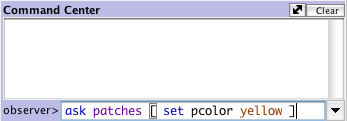
\includegraphics[width=8cm]{./imagenes/image1.png}
\end{center}

\item Pulse la tecla de retorno.

\paragraph{pregunta}¿Qué le pasó a la vista?
\subparagraph{respuesta}El fondo se ha vuelto amarillo

\paragraph{pregunta}¿Por qué los coches no se cambiaron también a amarillo?
\subparagraph{respuesta}Por qué el comando solo ordena a las parcelas la modificación de su color a amarillo

\paragraph{pregunta}¿Qué ocurrió en el Centro de Comando?
\subparagraph{respuesta}Se limpió el área de escritura y el programa guarda los comando en un historial

\begin{center}
	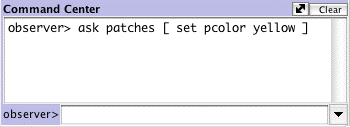
\includegraphics[width=8cm]{./imagenes/image2.png}
\end{center}

\item Escriba en el cuadro blanco en la parte inferior del Centro de Comando el texto que aparece a continuación:

\begin{center}
	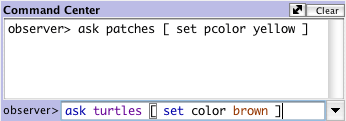
\includegraphics[width=8cm]{./imagenes/image3.png}
\end{center}


\paragraph{pregunta}Fue el resultado de lo que esperaba?
\subparagraph{respuesta}Le pide a las tortugas en nuestro caso coches que se cambien al color marrón

\begin{center}
	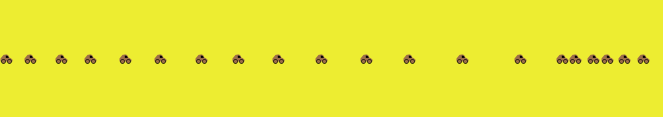
\includegraphics[width=8cm]{./imagenes/image4.png}
\end{center}

\item En el Centro de Comando, haga clic en el "observer>" en la esquina inferior izquierda:

\begin{center}
	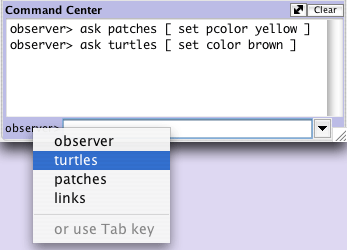
\includegraphics[width=8cm]{./imagenes/image5.png}
\end{center}


\item Elija "turtles" ("tortugas") en el menú emergente.
\item Escriba set color pink  y pulse retorno.
\item Pulse la tecla de tabulación hasta que vea "patches>" en la esquina inferior izquierda.
\item Escriba set pcolor white y pulse retorno.

\paragraph{pregunta}¿Cómo luce ahora la vista?

\begin{center}
	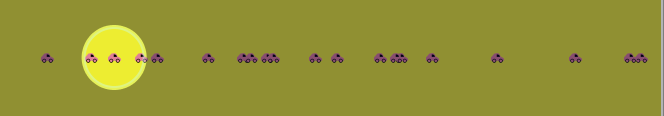
\includegraphics[width=8cm]{./imagenes/image6.png}
\end{center}

\paragraph{pregunta}¿Nota alguna diferencia entre estos dos comandos y los comando del observer anteriores?

\subparagraph{respuesta}Ya  no fue necesario especificar a qué actor le deseamos cambiar el color, todos los comandos que ejecutemos harán referencia al actor que se eligió en el menú

\hfill \\
El observador supervisa el mundo y, por tanto, puede dar un comando a los parches o las tortugas utilizando ask.  Al igual que en el primer ejemplo (observer> ask patches [set pcolor yellow]), el observador tiene que pedirle a los parches que fijen su pcolor en amarillo. Pero cuando un comando está dado directamente a un grupo de agentes al igual que en el segundo ejemplo (patches> set pcolor white), usted sólo tiene que dar el comando en sí.

\item Presione "setup".

\paragraph{pregunta}¿Qué pasó?
\subparagraph{respuesta}todo regreso a su estado inicial, debido a q el código está programado con esos colores y no los que modificamos.

\begin{center}
	TRABAJANDO CON COLORES
\end{center}

Sin duda notó en la sección anterior que usamos dos palabras diferentes para el cambio de color: color y pcolor.

\paragraph{pregunta}¿Cuál es la diferencia entre el color y pcolor?
\subparagraph{respuesta}Pcolor hace referencia a las parcelas y color hace referencia a las tortugas

\item Elija "turtles" en el menú desplegable del Centro de Comando (o utilice la tecla de tabulación).
\item Escriba set color blue y pulse retorno.

\paragraph{pregunta} ¿Qué pasó con los coches?
\subparagraph{respuesta}Ahora todos son azules sin distinción

\begin{center}
	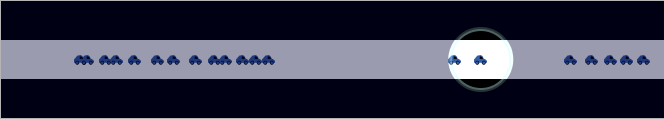
\includegraphics[width=8cm]{./imagenes/image7.png}
\end{center}


Piense en lo que hizo para volver los coches de color azul, y trate de poner los parches de color rojo.

\item En su lugar escriba set pcolor red y pulse retorno.

\begin{center}
	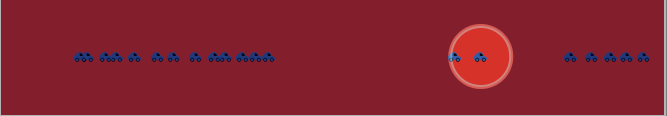
\includegraphics[width=8cm]{./imagenes/image8.png}
\end{center}

Para obtener un color que no tiene su propio nombre simplemente refiérase a él mediante un número, o añadiendo o restando un número a un nombre. Por ejemplo, escribir set color red, es la misma cosa que escribir set color 15. Usted puede conseguir una versión más clara o más oscura del mismo color usando, de la siguiente manera, un número que sea un poco mayor o un poco más pequeño.

\item Elija "patches" en el menú desplegable en el Centro de Comando (o utilice la tecla de tabulación).
\item Escriba set pcolor rojo - 2 (El espacio en torno a la "-" es importante.)

\begin{center}
	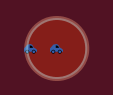
\includegraphics[width=8cm]{./imagenes/image9.png}
\end{center}

\item Escriba set pcolor rojo + 2

\begin{center}
	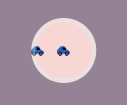
\includegraphics[width=8cm]{./imagenes/image10.png}
\end{center}

\begin{center}
	MONITORES DE AGENTE Y COMANDANTES DE AGENTE
\end{center}

\paragraph{pregunta}¿Cuál es el who number de la tortuga?
\subparagraph{respuesta:}2
\paragraph{pregunta}¿De qué color es esta tortuga?
\subparagraph{respuesta:}15
\paragraph{pregunta}¿De qué forma es esta tortuga?
\subparagraph{respuesta:}“car”

\item En el Comandante de Agente del monitor de turtle escriba set color pink para la tortuga 0.
\paragraph{pregunta}¿Qué sucede en la vista?
\subparagraph{respuesta:}La tortuga ahora es de color rosado o más específicamente 135
\paragraph{pregunta}¿Cambió algo en el monitor de la tortuga?
\subparagraph{respuesta:}El valor de color

\hfill \\

Una segunda forma de cambiar el color de una tortuga consiste en ir directamente a la variable color en el Monitor de la tortuga y cambiar allí directamente el valor.


\item Seleccione el texto a la derecha de "color" en el Monitor de Tortuga.
\item Escriba un nuevo color como green + 2.

\paragraph{pregunta}¿Qué pasó?
\subparagraph{respuesta}Color ahora es 57 y el auto es verde claro

 \hfill \\

La tercera forma de cambiar el color de una tortuga individual o de un parche es mediante el uso del observador. Dado que el observador supervisa el mundo NetLogo, este puede dar órdenes individuales que afectan a las tortugas así como a grupos de tortugas.

\item En el Centro de Comando, seleccione "observador" en el menú desplegable (o utilice la tecla de tabulación).

\item Escriba ask turtle 2 [set color blue] y pulse retorno.
\paragraph{pregunta}¿Qué sucede?
\subparagraph{respuesta}Todas las tortugas ahora son azules

\hfill \\

Al igual que hay Turtle Monitors (monitores de la tortuga), también hay Patch Monitors (monitores de Parches). Los monitores de parche trabajan muy similar a los monitores de tortuga.

\paragraph{pregunta}¿Puede hacer un monitor de parche y utilizarlo para cambiar el color de un solo parche?
\subparagraph{respuesta}Si es posible además se puede modificar otros valores.

\begin{center}
	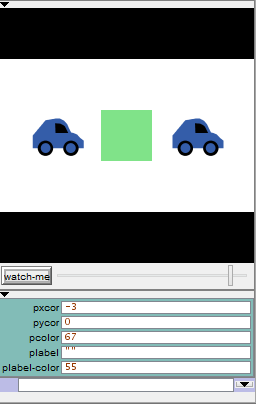
\includegraphics[width=8cm]{./imagenes/image11.png}
\end{center}

Recuerde, los parches están organizados en un sistema de coordenadas. Son necesarios dos números para trazar un punto en un gráfico: un valor en el eje "x"  y un valor para el eje "y". La localización de los parches está diseñada de la misma manera que el trazado un punto.

\item Abra un monitor del parche para cualquier parche.

\begin{center}
	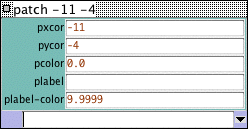
\includegraphics[width=8cm]{./imagenes/image12.png}
\end{center}

En la imagen el monitor muestra que en ese parche la variable pxcor  es -11 y su variable pycor  es -4. Si volvemos a la analogía del plano de coordenadas y quisiéramos trazar este punto, el punto podría ser encontrado en el cuadrante inferior izquierdo del plano coordenado donde x = -11 y = -4.

Para decirle a este parche en particular que cambie el color, use sus coordenadas.
En la parte inferior del monitor del parche ingrese set pcolor blue y pulse retorno.
Al escribir un comando en el monitor de una tortuga o de un parche, solo se modificará esa tortuga o ese parche.
También puede hablar con un único parche desde el Centro de Comando:
En el Centro de Comando, escriba ask patch -11 -4 [set pcolor green] y pulse retorno.


\begin{center}
	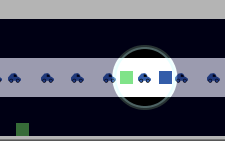
\includegraphics[width=8cm]{./imagenes/image13.png}
\end{center}


\end{itemize}


\end{document}




